\section{Модель линейной регрессии с выбросами при наличии группирования наблюдений}
Рассмотрим модель линейной регрессии:
\begin{eqnarray}
    &\label{eq2}y_i= 
    \begin{pmatrix}
        \beta_0\\
        \beta_1\\
        \dots\\
        \beta_n
    \end{pmatrix}\times
    \begin{pmatrix}
        1\\
        x_{i1}\\
        \dots\\
        x_{in}
    \end{pmatrix}^{T}+ \varepsilon_i,\\
    &y_i= f(x_i,\beta)+\varepsilon_i,\\
    &f(x_i,\beta)=\beta_0+\beta_1 x_{i1}+\beta_2 x_{i2}+\dots+\beta_n x_{in},
\end{eqnarray}
Здесь $y_i$ -- зависимая переменная, $x_i=(x_{i1},x_{i2},\dots,x_{in})$ -- вектор регрессоров, \{$\beta_k, k=\overline{0,n}$\}-- коэффициенты линейной регрессии, а $\varepsilon_i$ -- случайная ошибка $i$-го эксперимента, распределение которой подчиняется нормальному закону с нулевым математическим ожиданием и дисперсией $\sigma^2$, $N$-объем выборки.
Каждый $y_i$ принадлежит нормальному распределению:
\begin{eqnarray}
    \label{eq12} y_i=f(x_i,\beta)+\varepsilon_i \sim \mathcal{N}(f(x_i,\beta),\sigma^2).
\end{eqnarray}

Предполагается, что выборка содержит выбросы, описываемые следующими соотношениями.
\begin{eqnarray}
    \label{eq3}y_i^{\widetilde{\varepsilon}}=(\xi_i)y_i+ (1-\xi_i)\eta_i,
\end{eqnarray}
где $\xi_i$ принимает значение, равное 1, с вероятностью $1-\widetilde{\varepsilon}$ и значение, равное 0, с вероятностью $\widetilde{\varepsilon}$:
\begin{eqnarray}\label{eq4}
    \begin{cases}
        P\{\xi_i=0\}=\widetilde{\varepsilon},\\
        P\{\xi_i=1\}=1-\widetilde{\varepsilon},
    \end{cases},
\end{eqnarray}
$\eta_i$-случайная величина из некоторого вообще говоря неизвестного распределения.

Параметр $\xi_i$ имеет следующий содержательный смысл: если $\xi_i=0$, то вместо истинного значения мы наблюдаем выброс, если $\xi_i=1$, то наблюдается истинное значение.
Переменную $\widetilde{\varepsilon}$ будем называть долей аномальных наблюдений. Величины $\xi_i, x_i$ и $\eta_i$ являются независимыми.

Пусть множество значений функции регрессии, т.е множество $\mathbb{R}$, разбито на $k$ непересекающихся полуинтервалов:
\begin{eqnarray}
    \mathbb{R}=(-\infty,a_1]\bigcup(a_1,a_2]\bigcup \dots \bigcup(a_{k-1},+\infty ).
\end{eqnarray}
Полученные полуинтервалы будем обозначать: $\nu_0,\dots,\nu_{k-1}$.

Предполагается, что каждый раз вместо истинного значения зависимой переменной $y_i$ наблюдается только номер интервала, в который это наблюдение попало.
Тогда для каждого $y_i$ будем наблюдать лишь номер полуинтервала $\mu_i$, в который он попал.
\begin{eqnarray}
    \label{eq13}\mu_i=j, \textup{если $y_i$} \in \nu_j.
\end{eqnarray}

В таком случае принято говорить, что имеет место группирование наблюдений, а сами наблюдения называются группироваными \cite{OLSforGrouping}.

\newpage
\section{Статистическое оценивание параметров линейной регрессии с выбросами при наличии группирования наблюдений}
Введем обозначение для функции распределения стандартного нормального закона:
\begin{eqnarray}
    \Phi(x)=\frac{1}{\sqrt{2}\sigma}\int_{-\infty}^{x}e^{\frac{-t^2}{2}}dt.
\end{eqnarray}

Тогда функцию распределения нормального закона с параметрами $\mu,\sigma^2$ можно представить как:
\begin{eqnarray}
    \label{eq10}F(x)=\Phi(\frac{x-\mu}{\sigma}),
\end{eqnarray}
где $\sigma = \sqrt{\sigma^2}$. \hfill\break
Обозначим:
\begin{eqnarray}
    \textup{erf}(x)=\frac{2}{\sqrt{\pi}}\int_0^{x}e^{-t^2}dt.
\end{eqnarray}
Тогда:
\begin{eqnarray}
    \Phi(x)= \frac{1}{2} \Big[1+\textup{erf}\Big(\frac{x}{\sqrt{2}} \Big) \Big].
\end{eqnarray}
Подставив полученные выражения в (\ref{eq10}) получим:
\begin{eqnarray}
    F(x)= \frac{1}{2} \Big[1+\textup{erf}\Big(\frac{x-\mu}{\sqrt{2}\sigma} \Big) \Big].
\end{eqnarray}
При модельных предположениях (\ref{eq12}) вероятность попадания $y_i$ в полуинтервал $\nu_j$ равна:
\begin{multline}
    P\{y_i\in\nu_j\}= F_{y_i}(a_{j+1})-F_{y_i}(a_{j})=\\
    =\begin{cases}
        \frac{1}{2}(\textup{erf}(\frac{a_{j+1}-f(x_i,\beta)}{\sqrt{2}\sigma})-\textup{erf}(\frac{a_{j}-f(x_i,\beta)}{\sqrt{2}\sigma})),~j=\overline{1,k-2}\\
        \frac{1}{2}(1+\textup{erf}(\frac{a_{1}-f(x_i,\beta)}{\sqrt{2}\sigma})),~j=0\\
        \frac{1}{2}(1+\textup{erf}(\frac{a_{k-1}-f(x_i,\beta)}{\sqrt{2}\sigma})),~j=k-1
    \end{cases}.
\end{multline}
Понятно, что:
\begin{eqnarray}
    P(\mu_i=j)=P(y_i\in \nu_{\mu_i}).
\end{eqnarray}

Решается задача статистического оценивания параметров модели \{$\beta_k, k=\overline{0,n}$\} по известным группированным наблюдениям с аномалиями.

Для этого построим функцию правдоподобия:
\begin{eqnarray}
    \label{eq22}\label{eq23}&l(\beta,\sigma^2, \mu_1,\dots, \mu_{N})=\sum\limits_{i=1}^{N}\ln(P(y_i\in \nu_{\mu_i}))=\\
    &=\sum\limits_{i=1}^{N}\ln\begin{cases}
        \frac{1}{2}(\textup{erf}(\frac{a_{j+1}-f(x_i,\beta)}{\sqrt{2}\sigma})-\textup{erf}(\frac{a_{j}-f(x_i,\beta)}{\sqrt{2}\sigma})),~i=\overline{1,k-2}\\
        \frac{1}{2}(1+\textup{erf}(\frac{a_{1}-f(x_i,\beta)}{\sqrt{2}\sigma})),~i=0\\
        \frac{1}{2}(1+\textup{erf}(\frac{a_{k-1}-f(x_i,\beta)}{\sqrt{2}\sigma})),~i=k-1
    \end{cases},
\end{eqnarray}
где:
\begin{eqnarray}
    \textup{erf}(x)=\frac{2}{\sqrt{\pi}}\int_0^{x}e^{-t^2}dt.
\end{eqnarray}

Для максимизирования функции правдоподобия решим систему уравнений:
\begin{eqnarray}
    \label{eq24}\frac{\delta l}{\delta \beta}=0,
\end{eqnarray}
где:
\begin{multline}
    \label{eq27}\frac{\delta l}{\delta \beta}=\frac{\delta \sum\limits_{i=1}^{N}\ln P(y_i\in \nu_{\mu_i})}{\delta \beta}=~\\
    =\frac{\delta \sum\limits_{i=1}^{N} \ln(\frac{1}{2}(\textup{erf}(\frac{a_{\mu_i+1}-f(x_i,\beta)}{\sqrt{2}\sigma})-\textup{erf}(\frac{a_{\mu_i}-f(x_i,\beta)}{\sqrt{2}\sigma})) )         }{\delta \beta}=~\\
    =  \sum\limits_{i=1}^{N}\Big((1-(\delta_{\mu_i 0}+\delta_{\mu_i k-1}))\frac{(\textup{erf'}(\frac{a_{\mu_i+1}-f(x_i,\beta)}{\sqrt{2}\sigma})-\textup{erf'}(\frac{a_{\mu_i}-f(x_i,\beta)}{\sqrt{2}\sigma}))}{ (\textup{erf}(\frac{a_{\mu_i+1}-f(x_i,\beta)}{\sqrt{2}\sigma})-\textup{erf}(\frac{a_{\mu_i}-f(x_i,\beta)}{\sqrt{2}\sigma}))}+~\\
    +(\delta_{\mu_i 0}+\delta_{\mu_i k-1})\frac{\textup{erf'}(\frac{a_{\mu_i}-f(x_i,\beta)}{\sqrt{2}\sigma})}{(1+\textup{erf}(\frac{a_{\mu_i}-f(x_i,\beta)}{\sqrt{2}\sigma}))}\Big)  (-1) \frac{\delta f(x_i,\beta)}{\delta \beta} )=~
\end{multline}
\begin{multline}
    \nonumber 
    =-\sum_{i=1}^{N}\begin{pmatrix}
        1\\
        x_{i1}\\
        \dots\\
        x_{in}
    \end{pmatrix}\times  \Big((1-(\delta_{\mu_i 0}+\delta_{\mu_i k-1}))\frac{(\textup{erf'}(\frac{a_{\mu_i+1}-f(x_i,\beta)}{\sqrt{2}\sigma})-\textup{erf'}(\frac{a_{\mu_i}-f(x_i,\beta)}{\sqrt{2}\sigma}))}{ (\textup{erf}(\frac{a_{\mu_i+1}-f(x_i,\beta)}{\sqrt{2}\sigma})-\textup{erf}(\frac{a_{\mu_i}-f(x_i,\beta)}{\sqrt{2}\sigma}))}+~\\
    +(\delta_{\mu_i 0}+\delta_{\mu_i k-1})\frac{\textup{erf'}(\frac{a_{\mu_i}-f(x_i,\beta)}{\sqrt{2}\sigma})}{(1+\textup{erf}(\frac{a_{\mu_i}-f(x_i,\beta)}{\sqrt{2}\sigma}))}\Big) .
\end{multline}
$\delta_{ij}$ - символ Кронекера.

Известно приближение для функции $\textup{erf}(x)$:
\begin{eqnarray}
    (\textup{erf} x)^2&\approx& 1- \exp(-x^2 \frac{\frac{4}{\pi}+ax^2}{1+ax^2}),\\
    \nonumber a&=&\frac{8}{3\pi}\frac{3-\pi}{\pi -4}.
\end{eqnarray}
Оно считается достаточно точным для $x$ близких к $0$ и к $\infty$ \cite{Winitzki}. \hfill\break

Найдем производную для этого приближения:
\begin{eqnarray}
    \label{eq26}\textup{erf}'(x) = \exp(-x^2 \frac{\frac{4}{\pi}+ax^2}{1+ax^2}) \frac{-2x\frac{\frac{4}{\pi}+ax^2}{1+ax^2}+(2ax^3)\frac{\frac{4}{\pi}+ax^2}{1+ax^2}-\frac{2ax^3}{1+ax^2}}{2\sqrt{1- \exp(-x^2 \frac{\frac{4}{\pi}+ax^2}{1+ax^2})}}.
\end{eqnarray}

Уравнение (\ref{eq24}) решается методом секущих.


\subsection{Метод секущих}\label{sec4_2}
Так как мы не можем привести систему $ \frac{\delta l}{\delta \beta}=0$ к виду, удобному для итерации, то нам придется искать ее нули с помощью метода секущих.
Введем вектор ошибки $\check{\varepsilon}^{(k)}=\beta^{*}-\beta^{(k)}$. Тогда для его определения имеем:
\begin{eqnarray}
    \frac{\delta l (\beta^{(k)}+\check{\varepsilon}^{(k)})}{\delta \beta}=0.
\end{eqnarray}
Строя разложение левой части по формуле Тейлора и ограничиваясь лишь линейными членами\cite{NumericalMethods}, будем иметь систему:
\begin{eqnarray}
    \frac{\delta }{\delta \beta}\frac{\delta l (\beta^{(k)}}{\delta \beta}\Delta \beta^{(k)}=-\frac{\delta l (\beta^{(k)})}{\delta \beta}.
\end{eqnarray}
Вторая производная функции $l$ приближается с помощью выражения:
\begin{eqnarray}
    \frac{\delta }{\delta \beta_j}\frac{\delta l(\beta_1^{(k)},\dots, \beta_n^{(k)}) }{\delta \beta}\approx \frac{\frac{\delta l(\beta_1^{(k)},\dots,\beta_j^{(k)},\dots, \beta_n^{(k)}) (\beta^{(k)}}{\delta \beta}-\frac{\delta l(\beta_1^{(k)},\dots,\beta_j^{(k-1)},\dots, \beta_n^{(k)}) (\beta^{(k)}}{\delta \beta}}{\beta_j^{(k)}-\beta_j^{(k-1)}}.
\end{eqnarray}
Если матрица $\frac{\delta }{\delta \beta}\frac{\delta l (\beta^{(k)}}{\delta \beta}$ невырожденная (а в нашем случае она диагональная), то из этой системы можно единственным образом найти $\Delta \beta^{(k)}$ и построить приближение:
\begin{eqnarray}
    \beta^{(k+1)}=\beta^{(k)}+\Delta \beta^{(k)}.
\end{eqnarray}

\subsection{Переклассификая выборки}
Теперь имеем нули производной функции $l$, а также ее значения на границе отрезка $[a,b]$.
Переберем эти значения и таким образом найдем значение вектора $\hat{\beta}$, где она достигает своего максимального значения.

Для уменьшения влияния выбросов будем использовать переклассификацию выборки.
В ходе выполнения дипломной работы было испробовано несколько способов переклассификации выборки. Один из них: метод $K$ ближайших соседей. 

\subsubsection{Метод $K$ ближайших событий}
Идея заключается в том, что аномальные наблюдения с большей вероятностью попадают не в те интервалы, в которые попадают истинные наблюдения. 
При этом переклассификация может помочь отнести аномальные наблюдения к истинным классам и улучшить качество оценивания.

На первом этапе для каждого вектора $x_i$ имели класс $\mu_i$: т.е. пару $(x_i,\mu_i)$.
Далее выполним переклассификацию выборки. 
Для этого построим новую выборку такого же объема $N$.
Пройдемся по каждому элементу $(x_i, \mu_i)$ выборки и для этого наблюдения построим новое:
\begin{eqnarray}
    (x_i, \check{\mu}_i),
\end{eqnarray}
где $\check{\mu}_i$ получен по методу $K$-соседей.\hfill\break
\begin{eqnarray}
    \check{\mu}_i = \arg\max_j \sum_{k \in V_i,~k\neq i} \delta_{\check{\mu}_k j}~,
\end{eqnarray}
где $V_i$ множество индексов $l$ первых $K$ векторов $x_l$, отсортированных по возрастанию расстояния до вектора $x_i$.

После переклассификации выборки, к ней применяется функция правдоподобия из уравнений (\ref{eq22}), только теперь с использованием новых классов $\check{\mu}_i$ вместо $\mu_i$. 
Она аналогично максимизируется и в итоге находится новая оценка параметров $\hat{\beta}$.

В ходе экспериментов (раздел 3.2) оказалось, что метод $K$ ближайших соседей показывает слабо исправляет ошибочные классы в выборке, поэтому было решено использовать другой подход в переклассификации.

\subsubsection{Переклассификация с использованием Локального уровня выброса и Случайного леса}
Идея метода заключается в следующем: определим в выборке такие наблюдения, которые, вероятно, являются аномальными с помощью какого-либо способа. После этого выберем наблюдения, которые не определились как аномальные.
Обучим на полученных наблюдениях классификатор. После этого с помощью обученного классификатора переклассифицируем те наблюдения, которые определились как аномальные. В итоге получим выборку, которую будем использовать при решении уравнения (\ref{eq22}).

Для определения аномальных наблюдений можно использовать Локальный уровень выброса. Метод был предложен Маркусом М. Бройнигом, Гансом-Петер Кейгелем, Реймондом Т.~НГ и Ёргом Сандером в 2000 году. Аномальные наблюдения находятся с помощью измерения локального отклонения точек с учётом их соседей.
Метод основан на концепте локальной плотности достижимости, где локальная плотность достижимости вычисляется с учётом ближайших $K$ соседей, расстояние до которых используется для вычисления плотности. Сравнивая локальную плотность точки с локальной плотностью соседей можно определять точки, которые обладают значительно меньшей локальной плотностью по сравнению с соседями. Такие точки будем считать выбросами.

Пусть $x_i$ является некоторой точкой выборки. Определим $\rho(x_i, x_l)$ - расстояние от точки $x_i$ до точки $x_l$ (будем использовать меру Евклида), $\rho_k(x_i)$ - расстояние от точки $x_i$ до её $K$-го соседа. 
Аналогично методу $K$-ближайших соседей обозначим множество индексов $k$ первых $K$ векторов $x_k$, отсортированных по возрастанию расстояния до вектора $x_i$ через $V_i$.
Использользуя введеные величины зададим:
\begin{eqnarray}
    \hat{\rho}_k(x_i, x_l) = \max{\rho_k(x_l), \rho(x_i, x_l)}
\end{eqnarray}

Такую величину можно интерпретировать как истинное расстояние от точки $x_l$ до точки $x_i$ если $x_l$ не входит в ее $K$ ближайших соседей или расстояние до точки $x_{V_{l_K}}$ в противном случае. 
Данная величина введена для того, чтобы более стабильно вычислять расстояние для тех значений, которые входят в $K$-соседей точки $x_l$. 

Заметим, что введенная величина не обладает свойством симметричности.

Локальную плотность достижимости зададим выражением:
\begin{eqnarray}
    \textup{lrd}_k(x_i) = 1 / \bigg(\frac{\sum\limits_{l\in V_i}\hat{\rho}_k(x_i, x_l)}{|V_i|}\bigg)
\end{eqnarray}

Теперь можно задать величину:
\begin{eqnarray}
    \textup{LOF}_k(x_i) = \frac{\sum\limits_{l\in V_i}\frac{\textup{lrd}_k(x_l)}{\textup{lrd}_k(x_i)}}{|V_i|}
\end{eqnarray}
Она является средней локальной плотностью достижимости соседей точки $x_i$ по отношению к своей локальной плотности достижимости точки $x_i$. 

По полученному значению можно судить, является ли наблюдение $x_i$ выбросом или нет:
\begin{itemize}
    \item $\textup{LOF}_k(x_i)\sim 1$   - означает, что такая же плотность как у соседей\\
    \item $\textup{LOF}_k(x_i)<1$  - означает, что большая плотность чем у соседей (наблюдение - истинное)\\
    \item $\textup{LOF}_k(x_i)>1$ - означает, что меньшая плотность чем у соседей (наблюдение - выброс) 
\end{itemize}

\newpage
\subsection{Альтернативные оценки параметров модели}
Рассмотрим альтернативный метод оценивания параметров модели регрессии, основанный на замене группированных наблюдений серединами соответствующих интервалов. 
Такой метод встречается в литературе, например в \cite{interval_valued}.

Метод заключается в следующем:
пусть имеется $\mu_i$ - номер полуинтервала, в который попало очередное наблюдение $y_i$. Ему соответствует полуинтервал $\nu_{\mu_i}$ (из (\ref{eq13})), т.е. полуинтервал:
\begin{eqnarray}
    y_i\in (a_{\nu_{\mu_i}},a_{\nu_{\mu_i}+1}], i = \overline{1,N}
\end{eqnarray}
(считаем что $a_1<y_i<a_{k-1}, i=\overline{1,N}$, т.е $1\leq\mu_i\leq k-2$).

Найдем центральную точку этого интервала, т.е. точку
\begin{eqnarray}
    \check{y_i} = \frac{a_{\nu_{\mu_i}} + a_{\nu_{\mu_i}+1}}{2}.
\end{eqnarray}

Построим для всех значений функции регрессии $y_i$ значения $\check{y_i}$.
Будем использовать в качестве значений функции регрессии полученные значения $\check{y_i}$, а в качестве регрессоров $x_i$ и построим МНК оценки параметров $\beta$.

Теперь имеет три вида оценок: оценки максимального правдоподобия, оценки максимального правдоподобия с переклассификацией, МНК по серединам интервалов. 
\newpage
\subsection{Полиномиальная регрессия}
Введем теперь модель полиномиальной регрессии.

\begin{equation}
    \begin{array}{c}
        \label{eq28}y_i=\beta_0+\beta_1 x_{i1}^1+\beta_2 x_{i2}^2+\dots+\beta_n x_{in}^n+\varepsilon_i, i=\overline{1,N},\\
        y_i = \sum\limits_{l=1}^{n} x_{il}^{l-1} + \varepsilon_i, i=\overline{1,N},\\
        y_i= f(x_i,\beta)+\varepsilon_i,\\
        f(x_i,\beta)=\beta_0+\beta_1 x_{i1}^1+\beta_2 x_{i2}^2+\dots+\beta_n x_{in}^n
    \end{array}
\end{equation}
В случае полиномиальной регрессии также справедливо:
\begin{eqnarray}
    y_i=f(x_i,\beta)+\varepsilon_i \sim \mathcal{N}(f(x_i,\beta),\sigma^2).
\end{eqnarray}

Поскольку оценки строились путём максимизирования функции:
\begin{eqnarray}
    &l(\beta,\sigma^2, \nu_0,\dots, \nu_{k-1})=\sum_{i=1}^{N}\ln(P(y_i\in \nu_{\mu_i}))=\\
    &=\sum\limits_{i=1}^{N}\ln\begin{cases}
        \frac{1}{2}(\textup{erf}(\frac{a_{j+1}-f(x_i,\beta)}{\sqrt{2}\sigma})-\textup{erf}(\frac{a_{j}-f(x_i,\beta)}{\sqrt{2}\sigma})),~i=\overline{1,k-2}\\
        \frac{1}{2}(1+\textup{erf}(\frac{a_{1}-f(x_i,\beta)}{\sqrt{2}\sigma})),~i=0\\
        \frac{1}{2}(1+\textup{erf}(\frac{a_{k-1}-f(x_i,\beta)}{\sqrt{2}\sigma})),~i=k-1
    \end{cases},
\end{eqnarray}
а функция правдоподобия максимизировалась путём решения системы уравнений:
\begin{eqnarray}
    \frac{\delta l}{\delta \beta}=0,
\end{eqnarray}
которая примет вид:
\begin{multline}
    \frac{\delta l}{\delta \beta}=\frac{\delta \sum\limits_{i=1}^{N}\ln P(y_i\in \nu_{\mu_i})}{\delta \beta}=~\\
    =\frac{\delta \sum\limits_{i=1}^{N} \ln(\frac{1}{2}(\textup{erf}(\frac{a_{\mu_i+1}-f(x_i,\beta)}{\sqrt{2}\sigma})-\textup{erf}(\frac{a_{\mu_i}-f(x_i,\beta)}{\sqrt{2}\sigma})) )         }{\delta \beta}=~\\
    =  \sum\limits_{i=1}^{N}\Big((1-(\delta_{\mu_i 0}+\delta_{\mu_i k-1}))\frac{(\textup{erf'}(\frac{a_{\mu_i+1}-f(x_i,\beta)}{\sqrt{2}\sigma})-\textup{erf'}(\frac{a_{\mu_i}-f(x_i,\beta)}{\sqrt{2}\sigma}))}{ (\textup{erf}(\frac{a_{\mu_i+1}-f(x_i,\beta)}{\sqrt{2}\sigma})-\textup{erf}(\frac{a_{\mu_i}-f(x_i,\beta)}{\sqrt{2}\sigma}))}+~\\
    +(\delta_{\mu_i 0}+\delta_{\mu_i k-1})\frac{\textup{erf'}(\frac{a_{\mu_i}-f(x_i,\beta)}{\sqrt{2}\sigma})}{(1+\textup{erf}(\frac{a_{\mu_i}-f(x_i,\beta)}{\sqrt{2}\sigma}))}\Big)  (-1) \frac{\delta f(x_i,\beta)}{\delta \beta} )=~
\end{multline}
\begin{multline}
    \nonumber 
    =-\sum_{i=1}^{N}\begin{pmatrix}
        1\\
        x_{i1}^1\\
        \dots\\
        x_{in}^n
    \end{pmatrix}\times  \Big((1-(\delta_{\mu_i 0}+\delta_{\mu_i k-1}))\frac{(\textup{erf'}(\frac{a_{\mu_i+1}-f(x_i,\beta)}{\sqrt{2}\sigma})-\textup{erf'}(\frac{a_{\mu_i}-f(x_i,\beta)}{\sqrt{2}\sigma}))}{ (\textup{erf}(\frac{a_{\mu_i+1}-f(x_i,\beta)}{\sqrt{2}\sigma})-\textup{erf}(\frac{a_{\mu_i}-f(x_i,\beta)}{\sqrt{2}\sigma}))}+~\\
    +(\delta_{\mu_i 0}+\delta_{\mu_i k-1})\frac{\textup{erf'}(\frac{a_{\mu_i}-f(x_i,\beta)}{\sqrt{2}\sigma})}{(1+\textup{erf}(\frac{a_{\mu_i}-f(x_i,\beta)}{\sqrt{2}\sigma}))}\Big),
\end{multline}
то построенные оценки также применимы и для полиномиальной регрессии.

Также как и в случае линейной регрессии считаем, что выборка содержит выбросы, т.е., аналогично:
\begin{eqnarray}
    y_i^{\widetilde{\varepsilon}}=(\xi_i)y_i+ (1-\xi_i)\eta_i,
\end{eqnarray}
здесь $y_i$ задаются формулой (\ref{eq28}).

\newpage
\section{Компьютерные эксперименты}
% \subsection{Параметры модели и оценок}
% В ходе экспериментов использовались следующие параметры модели:
% \begin{center}
%     \begin{tabular}{|p{5cm}|p{5cm}|}
%         \hline
%         \multicolumn{2}{|c|}{Параметры программы} \\
%         \hline
%         Переменная&значение\\
%         \hline
%         Размер выборки $N$& 1000\\
%         \hline
%         Доля выбросов $\widetilde{\varepsilon}$& 0.08\\
%         \hline
%         Параметры регрессии $\beta$& $(90,4)$\\
%         \hline
%         Регрессоры $x_i$ & $\sim U(-5,5)$\\
%         \hline
%         $\varepsilon_i$&$\sim N(0,16)$\\
%         \hline
%         $\eta_i$&$\sim N(100,100)$\\
%         \hline
%         Величина $K$ из пункта 2.3 курсового проекта &$10$\\
%         \hline
%     \end{tabular},
% \end{center}
% \newpage

\subsection{Сравнительный анализ построенной оценки с альтернативной}
\subsubsection{Эксперимент с изменением объема выборки}
В следующем эксперименте был произведен сравнительный анализ вариаций ОМП-оценок с МНК оценками в зависимости от объема выборки.

Объем выборки $N$ изменялся от $N_1=100$ до $N_2=500$, при этом выборка дополнялась, а не генерировалась новая. Использовалась модель линейной регрессии. Доля выбросов была постоянна и равнялась $\widetilde{\varepsilon}=0.08$. Параметры регрессии были постоянными и равнялись $\beta=(90,4)^T$. 
Регрессоры $x_i$ были из равномерного распределения $U(-5,5)$, ошибки эспериментов $\varepsilon_i\sim \mathcal{N}(0,16)$.

\begin{center}
    \captionof{table}{Параметры модели и оценок}\label{tab1}
    \begin{tabular}{|p{5cm}|p{5cm}|}
        \hline
        \multicolumn{2}{|c|}{Параметры программы} \\
        \hline
        Переменная&значение\\
        \hline
        Размер выборки $N$& от 100 до 500\\
        \hline
        Доля выбросов $\widetilde{\varepsilon}$& 0.08\\
        \hline
        Параметры регрессии $\beta$& $(90,4)$\\
        \hline
        Регрессоры $x_i$ & $\sim U(-5,5)$\\
        \hline
        $\varepsilon_i$&$\sim \mathcal{N}(0,16)$\\
        \hline
        $\eta_i$&$\sim \mathcal{N}(100,100)$\\
        \hline
        Величина $K$  &$10$\\
        \hline
    \end{tabular},
\end{center}
\begin{figure}[h!]
    \centering
    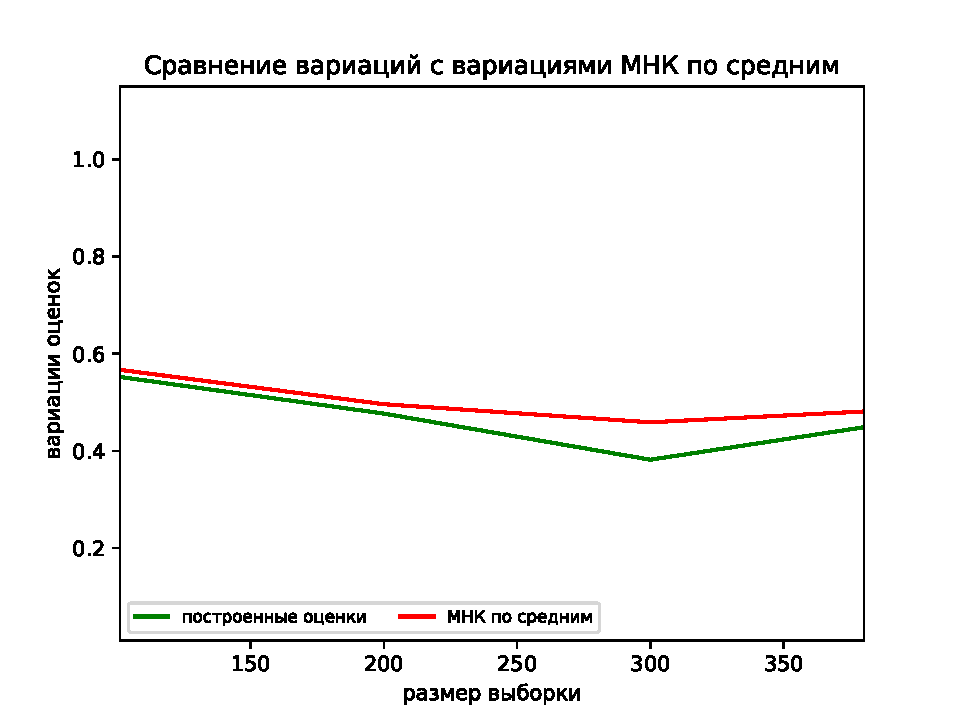
\includegraphics[width=100mm]{../images/OLS_GEM.pdf}
    \caption{Сравнение вариаций оценок\label{overflow}}
    \label{pic0}
\end{figure}
При сравнении графиков вариаций (рис.\ref{pic0}) можно сделать вывод, что ОМП дают лучший результат, 

\subsubsection{Эксперимент с полиномиальной регрессией}
Был проведен эксперимент с полиномиальной регрессией. Использовались те же параметры модели (таблица \ref{tab1}), объем выборки $N$ изменялся от 100 до 1000:
\begin{figure}[h!]
    \centering
    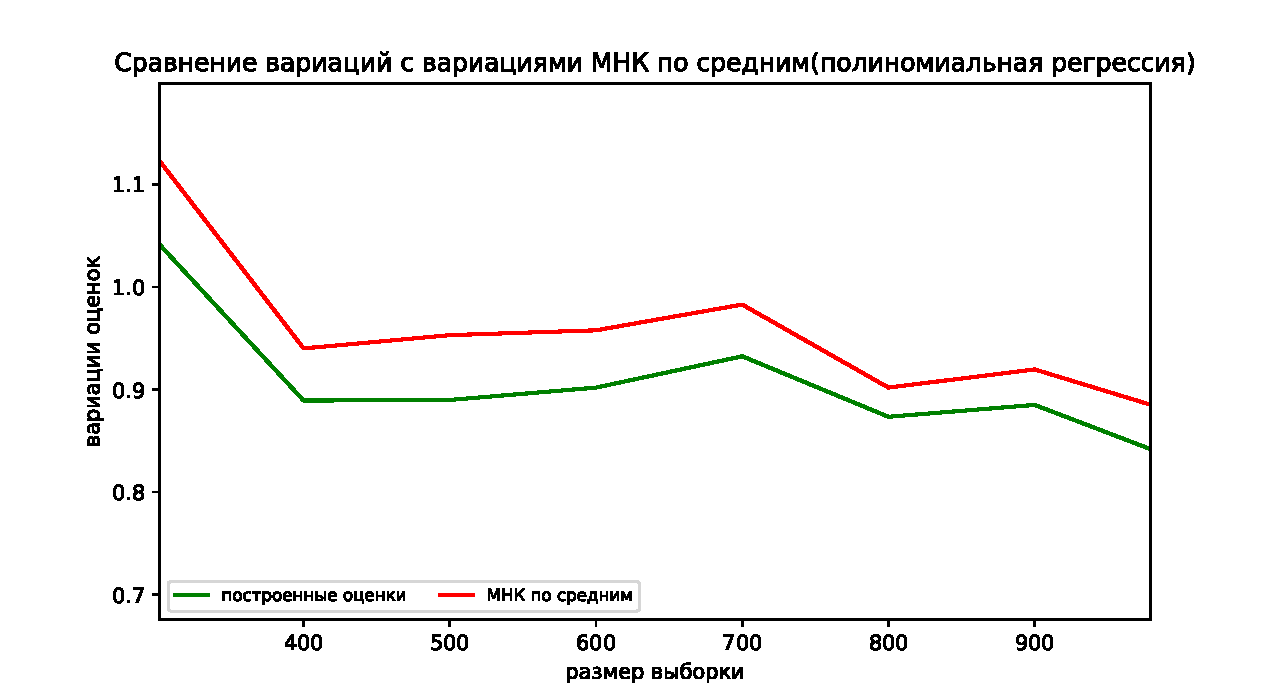
\includegraphics[width=150mm]{../images/polynomial.pdf}
    \caption{Вариации оценок в случае полиномиальной регрессии\label{overflow}}
    \label{pic3}
\end{figure}

Оба метода имели схожее поведение при изменении объема выборки, но построенные оценки максимального правдоподобия стабильно показывали лучший результат.

\newpage
\subsection{Эксперименты с изменением уровня переклассификации выборки}\label{ss3_3_1}
В ходе преддипломной практики были построены эксперименты с изменением величины K для метода $K$-ближайших соседей, используемого в переклассификации.  

Объем выборки $N$ был постоянным: $N=500$. Использовалась модель линейной регрессии. Доля выбросов была постоянна и равнялась $\widetilde{\varepsilon}=0.08$. Параметры регрессии были постоянными и равнялись $\beta=(90,4)^T$. 
Регрессоры $x_i$ были из равномерного распределения $U(-5,5)$, ошибки эспериментов $\varepsilon_i\sim \mathcal{N}(0,16)$. Величина $K$ менялась от $10$ до $40$.
\begin{center}
    \captionof{table}{Параметры модели и оценок экспериментов с переклассификацией выборки}\label{tab1}
    \begin{tabular}{|p{5cm}|p{5cm}|}
        \hline
        \multicolumn{2}{|c|}{Параметры программы} \\
        \hline
        Переменная&значение\\
        \hline
        Размер выборки $N$& 500\\
        \hline
        Доля выбросов $\widetilde{\varepsilon}$& 0.08\\
        \hline
        Параметры регрессии $\beta$& $(90,4)$\\
        \hline
        Регрессоры $x_i$ & $\sim U(-5,5)$\\
        \hline
        $\varepsilon_i$&$\sim \mathcal{N}(0,16)$\\
        \hline
        $\eta_i$&$\sim \mathcal{N}(100,100)$\\
        \hline
        Величина $K$  &от $10$ до $40$\\
        \hline
    \end{tabular},
\end{center}

\begin{figure}[h!]
    \centering
    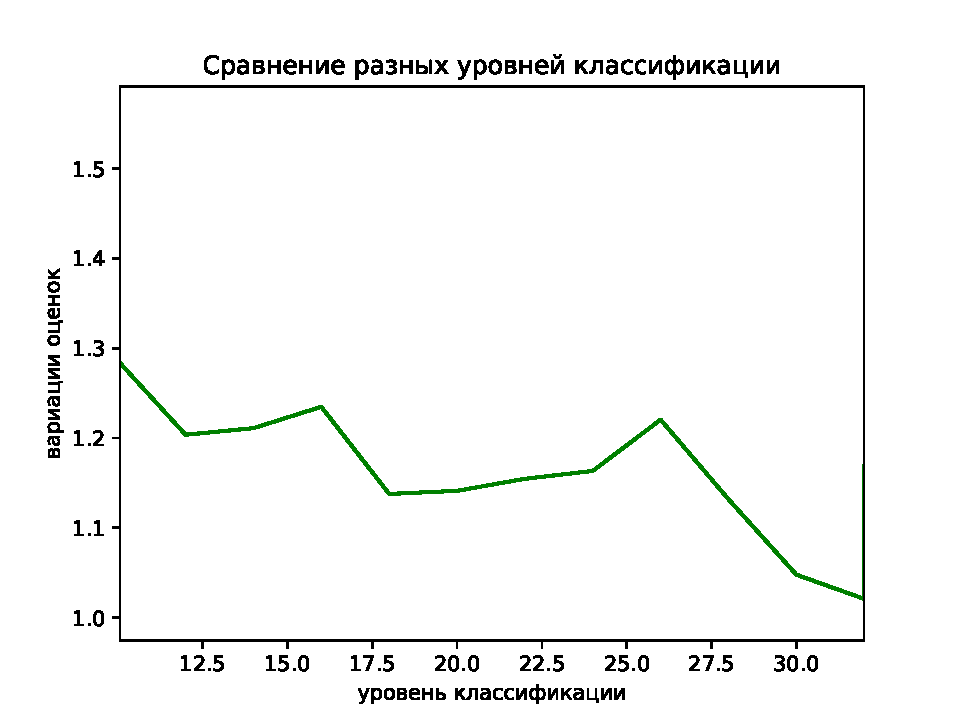
\includegraphics[width=100mm]{../images/different_recl_level.pdf}
    \caption{Зависимость вариаций от $K$ -- числа соседей, используемого в переклассификации выборки\label{overflow}}
    \label{pic1}
\end{figure}

В результате получилось, что при увеличении константы K точность оценки параметров растёт. 
\subsection{Сравнение вариаций с оценками без переклассификации}
Были проведены эксперименты для сравнения эмпирической вариации оценок максимального правдоподобия, когда использовалась вышеописанная переклассификация и когда не использовалась. При этом на каждой итерации выборка увеличивалась. 

Объем выборки $N$ изменялся от $N_1=100$ до $N_2=400$, при этом выборка дополнялась, а не генерировалась новая. Использовалась модель линейной регрессии. Доля выбросов была постоянна и равнялась $\widetilde{\varepsilon}=0.08$. Параметры регрессии были постоянными и равнялись $\beta=(90,4)^T$. 
Регрессоры $x_i$ были из равномерного распределения $U(-5,5)$, ошибки эспериментов $\varepsilon_i\sim \mathcal{N}(0,16)$. В методе, где использовалась переклассификация, величина $K$ выбиралась: $K=10$.
\vspace{3cm}
\begin{center}
    \captionof{table}{Параметры модели и оценок экспериментов}\label{tab1}
    \begin{tabular}{|p{5cm}|p{5cm}|}
        \hline
        \multicolumn{2}{|c|}{Параметры программы} \\
        \hline
        Переменная&значение\\
        \hline
        Размер выборки $N$& от 100 до 400\\
        \hline
        Доля выбросов $\widetilde{\varepsilon}$& 0.08\\
        \hline
        Параметры регрессии $\beta$& $(90,4)$\\
        \hline
        Регрессоры $x_i$ & $\sim U(-5,5)$\\
        \hline
        $\varepsilon_i$&$\sim \mathcal{N}(0,16)$\\
        \hline
        $\eta_i$&$\sim \mathcal{N}(100,100)$\\
        \hline
        В методе, с переклассификацией величина $K$& 10\\
        \hline
    \end{tabular},
\end{center}
\newpage
\begin{figure}[ht!]
    \centering
    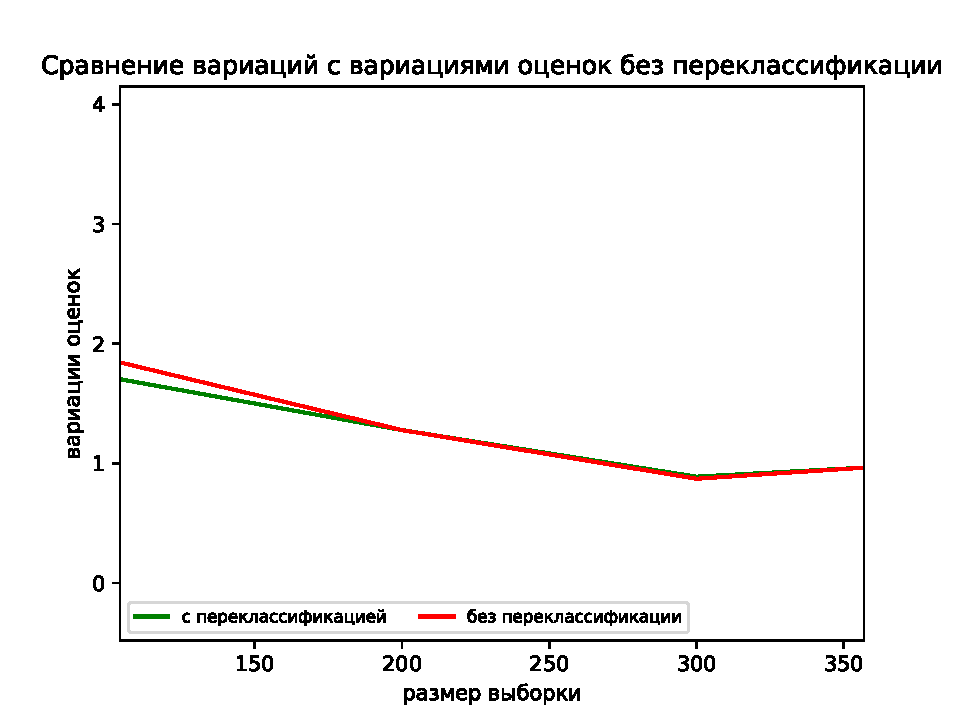
\includegraphics[width=100mm]{../images/on_off_recl.pdf}
    \caption{Сравнение вариаций оценок когда используется и не используется переклассификация\label{overflow}}
    \label{pic2}
\end{figure}

\newpage
